\chapter{Introduction}

Clouds represent one of the largest sources of uncertainty in estimating global
climate sensitivity \citep{williams2017}. Clouds over the ocean
are especially important for determining the radiation budget, due to the
low albedo of the sea surface compared to land.
Over the Southern Ocean (SO),
cloud cover exceeds 80\%, with predominantly boundary layer clouds \citep{mace2009}.
Due to its large influence on circulation and atmospheric transports in the
Southern Hemisphere, the SO is important for global climate. Unlike
most other places on the globe, it is largely unaffected by sources of
continental and anthropogenic aerosols, is dominated by a strong circumpolar
vortex, and its southern boundary is a permanently ice-covered continent,
which could mean that global parametrisations do not apply very well in this
region.
SO south of 30$^\circ$S accounts for about 43\% of anthropogenic CO$_2$ and 75%
of excess heat uptake \citep{frolicher2015}.
Observations in the SO are sparse, which limits the accuracy
of simulations by numerical weather prediction (NWP) models and general
circulation models (GCMs).
Globally, clouds have a predominantly cooling effect on the climate due to reflection
of sunlight, which exceeds the warming effect due to absorption of thermal
radiation from the surface, estimates identify 18 Wm$^{-2}$ of cooling relative to a cloud-free atmosphere
\citep{zelinka2017}. This effect is about 5 times as large as heating from
a doubling of CO$_2$, which highlights the importance of cloud cover in modulating
global climate. Nearly all climate models predict cloud feedback to be positive,
i.e. amplification of warming with increasing CO$_2$ concentration.

\begin{figure}[t]
\centering
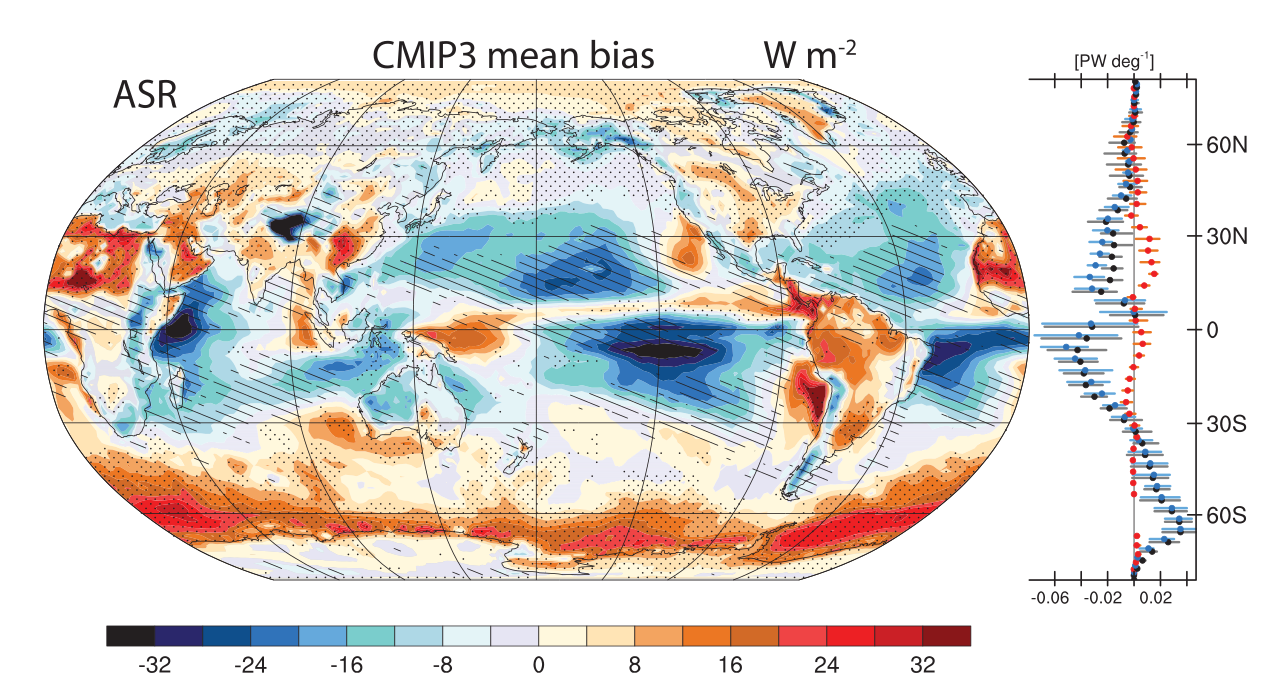
\includegraphics[width=\textwidth]{fig/trenberth-fassulo-sw-bias.png}
\caption[Biases in the TOA net radiation down]{
Biases in the TOA net radiation down relative to observations regionally for
1990--99
in $Wm^{-2}$, where stippled (hatched) regions correspond to regions
in which at least three quarters of the models share a common
positive (negative) bias. (right) The model zonal mean is given
(dots) with the 25th to 75th percentile range (lines) over land (red),
ocean (blue), and all (black) surfaces. \textbf{Adopted from
\cite{trenberth2010}.}
}
\label{fig:trenberth-fassulo-sw-bias}
\end{figure}

Shortwave (SW) radiation bias over the SO of up to 30 Wm$^{-2}$ is a
well-documented problem in current NWP models and GCMs
\citep{trenberth2010} (Fig. \ref{fig:trenberth-fassulo-sw-bias}),
and it has been the subject of many studies.
It manifests both as a bias in SW radiation reaching the surface and as a
SW reflectivity bias at the top of atmosphere (TOA).
\cite{bodas-salcedo2014} evaluated SW bias in a number
of GCMs and found a strong SW bias is a very common problem, leading to
overestimated sea surface temperature (SST) in the SO.
\cite{trenberth2010} noted that a poor representation of clouds might lead to
unrealistic projections for the Southern Hemisphere. This bias is linked to
large-scale model errors such as a double-intertropical
convergence zone \citep{hwang2013}, position of the midlatitude jet and
meridional energy transport \citep{mason2014}.
The reasons for the observed SW radiation bias
can be numerous, concurrent and compensating.
As noted by \cite{kelleher2019}, cloud biases in the SO can arise either
as a result of biases in large-scale dynamics, or cloud parametrisation.
To summarise, they can range
from microphysical to large-scale dynamics and be due to misrepresentation of:
cloud fraction, cloud optical depth, frequency of cloud regimes or types,
cloud vertical distribution and overlap, cloud horizontal distribution
and homogeneity, cloud phase and supercooled liquid content, surface albedo
(sea ice vs. water), moisture fluxes, large-scale circulation, extratropical
and polar cyclones, weather regimes, direct and indirect aerosol effects,
radiative transfer parametrisation, boundary layer turbulence and convection,
among others.

The New Zealand Earth System Model (NZESM)
is a relatively new earth system model based on the UK climate model HadGEM/UK Earth System Model (UKESM)
\citep{williams2016}, whose aim is to improve climate predictions for
Aotearoa/New Zealand. Reducing SO model biases is essential for
achieving this aim. \cite{walters2017}
showed that a clear and extensive SW radiation bias over the SO
is present in the atmospheric component of the model Global Atmosphere version 6.0 (GA6.0) compared to satellite
radiation budget observations by the Clouds and the Earth's Radiant Energy
System (CERES) \citep{wielicki1996}. The bias in the context of the UK Met Office
models has been studied by \cite{bodas-salcedo2012} by assessing cloud
regimes in cyclones.
Using observations by the International Satellite Cloud Climatology Project
(ISCCP) \citep{rossow1999},
Multi-angle Imaging SpectroRadiometer (MISR) \citep{diner1998}, Moderate Resolution Imaging Spectroradiometer (MODIS) \citep{salomonson2002},
Cloud-Aerosol Lidar and Infrared Pathfinder Satellite Observation
(CALIPSO) \citep{winker2010} and CloudSat \citep{stephens2002} satellites,
they found that the model underestimates optical depth of stratocumulus and
mid-topped clouds. Recently, \cite{davies2017} studied boundary layer
clouds in the SO compared to the Northern Hemisphere,
with a focus on supercooled liquid in clouds and cloud homogeneity.
They noted that boundary layer clouds are a likely explanation for the bias
due to their large fractional coverage over the SO.
Examination of cloud cover in the NZESM against passive satellite instruments
was performed by \cite{schuddeboom2017,schuddeboom2019} and is an ongoing effort.

While some authors focused on cloud distribution, others
emphasised the role of microphysics, especially supercooled liquid content.
Because supercooled liquid has a higher SW reflectivity than the equivalent amount
of ice particles (in terms of mixing ratio), it has a positive effect on cloud albedo.
\cite{morrison2011} studied the occurrence of supercooled liquid in clouds
over the SO using observations by MODIS and
found that it is present year-round in low clouds at temperature as low as
--40 $^{\circ}$C.
\cite{lawson2014} noted that supercooled liquid is often
underestimated in the Antarctic in GCMs, and mixed clouds can occur at
--32 $^{\circ}$C.
They showed that increasing supercooled liquid in the
Community Earth System Model (CESM) leads to a cloud radiative effect (CRE)
increase of 7.4 Wm$^{-2}$ over Antarctica. More recently, \cite{kay2016}
managed to fix the SW radiation bias in the CESM by increasing supercooled liquid
in shallow convective clouds, and notably they also needed to reduce a
compensating tropical SW radiation bias to maintain global radiation balance
in the model.
\cite{bodas-salcedo2016} found supercooled liquid to be abundant in
the SO in summer and contribute about 30\% to the reflected
SW radiation.
\cite{noh2019} developed an algorithm for detecting mixed-phase cloud with
liquid top in the SO using Himawari geosynchronous (GEO) satellite data, which are thought
to be common in the region, but difficult to detect with passive satellite
instruments. They focused on liquid‐top mixed‐phase clouds. In their case studies, they found both supercooled liquid
and mixed clouds with liquid top over the SO south of Australia and
New Zealand and noted that their algorithm may complement active instruments
in detecting mixed cloud.

Several field campaigns were performed in the SO in recent years:
Clouds, Aerosols, Precipitation, Radiation, and Atmospheric Composition over the Southern Ocean (CAPRICORN) \citep{mace2018a,mace2018b}, Measurements of Aerosols, Radiation and Clouds over the Southern Ocean (MARCUS) \citep{mcfarquhar2016},
the Southern Ocean Clouds, Radiation, Aerosol Transport Experimental Study (SOCRATES) \citep{mcfarquhar2014} and the Macquarie Island Cloud and Radiation Experiment (MICRE) \citep{demott2018}.
The SOCRATES campaign consisted of 15 flights of GV HIAPER and a voyage
of R/V Investigator from Hobart, Tasmania in January--February 2018,
organised by the National Science Foundation (NSF) and the
National Center for Atmospheric Research (NCAR). \cite{gettelman2020}
analysed cloud microphysical observations from these flights compared
to nudged CAM6 simulations, and found that CAM6 represents cloud properties
relatively well, and observed supercooled liquid clouds extensively in cold
sectors of cyclones. They found the representation of supercooled liquid
better than in CAM5 due to a scheme dependence on the available ice nuclei.
They found 50\% differences in ice water path (IWP) and liquid water path (LWP)
between CAM5 and CAM6. Their model simulates cloud droplet size distribution
prognostically and they found a satisfactory agreement with the in situ
airborne observations.
\cite{mace2018a} analysed cloud observations collected on the second CAPRICORN
voyage of R/V Investigator from Hobart, Tasmania to 53$^\circ$ S in March--April 2016.
In their radar and lidar observations, low cloud below 2 km was predominant
during the voyage and the total lidar cloud fraction was 76\%, compared to 87\%
in CloudSat--CALIPSO in the region and time of year in 2007--11, with
more high clouds identified by CloudSat--CALIPSO.
They also found that about 30\% of cloud is detected by a ship-based lidar but not
a radar due to low sensitivity of the radar. In terms of cloud phase,
they found that ice-phase processes occur 20-40\% more often than implied
by CALIPSO due to attenuation of the signal at the cloud top. Thus, one should
perhaps be cautious when using active satellite
products as a reference for supercooled liquid cloud evaluation in GCMs
in this region. They performed 1--2 daily soundings and found MERRA-2 about
1.2 K warmer and 8\% drier. They note that unlike the lidar, the radar is unable
to reliably detect cloud base height due to frequent precipitation, which
cannot be distinguished from cloud.
\cite{mace2018b} studied stratocumulus clouds occurring during the CAPRICORN
voyage. They characterise them as tenuous, supercooled, rarely drizzling
and present in cold air advection. They quantify their water path at 15--25 \unit{gm^{-2}},
effective radius at 8 \unit{\mu m}, number concentration at 20 \unit{cm^{-2}} and optical
depth 3--4. It is probably notable, however, that these values can be different
in the high-latitude SO, not reached by the CAPRICORN voyage. They hypothesise
that these non-precipitating stratocumulus clouds are responsible for majority
of the SO shortwave radiation biases identified in GCMs.
The MARCUS field campaign was conducted between November 2017 and March 2018
on \textit{Aurora Australis}. It was focused on collecting biogenic INP concentrations in the region,
but a range of ARM instruments were deployed on this ship.
\cite{zheng2019} analysed warm air advection events on the voyages and found
that they induce highly-stratified cloud-topped marine boundary layer with
stratiform clouds.

Multiple observational datasets are available for assessing the SO biases,
largely consisting of satellite datasets, and a relatively few ship- and
land-based datasets due to the very large costs and operational difficulties
of field campaigns in this remote and extreme-weather region. 
Satellite observations provide the most complete record both spatially and
temporally, although they do not provide historical records prior to
1960s and past observations are limited by instrument capabilities and
the availability of derived products. They have been utilised by most studies
of clouds in the SO and globally. Satellite instruments are very diverse, though only a few
datasets are readily available for studying clouds.
Operational GEO satellites provide near-continuous temporal
coverage,
which makes them ideal for studying clouds, but they have a limited use in
high-latitude regions such as the SO. In combination with operational polar-orbiting
low Earth orbit (LEO) satellites such as the NASA
Polar Operational Environmental Satellites (POES),
they have been used to produce a very long-term (1983--present) cloud-oriented
dataset ISCCP
\citep{schiffer1983}. However, this dataset is limited by
a small number of spectral channels of the Advanced Very High Resolution Radiometer
(AVHRR). Other extensive
cloud datasets include MODIS
on board of the NASA Afternoon Train (A-Train) satellites Aqua and Terra
and the Extended AVHRR Polar Pathfinder (APP-x) \citep{meier1997}. Other notable instruments available
for studying clouds include MISR
and passive
microwave sensors, due to their ability to observe cloud liquid water,
total column water vapour, vertically-resolved temperature profile, and
ability to see through clouds, even though their relatively low spatial
resolution makes passive microwave instruments less popular than passive visible (VIS) and infrared (IR)
instruments.
Passive VIS and IR satellite observations of clouds are ideal due to their high
spatial and temporal resolution, but have a number problems globally and some
specifically in polar latitudes \citep{bromwich2012}:

\begin{itemize}
\item Passive instruments can only observe the highest layer of clouds, unless
the layer is semi-transparent, meaning that cloud vertical structure is
poorly measured with passive instruments.
\item It is difficult to discern clouds from surface ice and snow
in the VIS spectrum due to similar albedo and in the IR
spectrum due to similar
temperature and frequent inversions.
\item Poor detection of semi-transparent high clouds, falsely classified as
mid-level clouds \citep{haynes2011}.
\item Lack of sunlight limits polar wintertime SW measurements.
\end{itemize}

\begin{figure}[t]
\centering
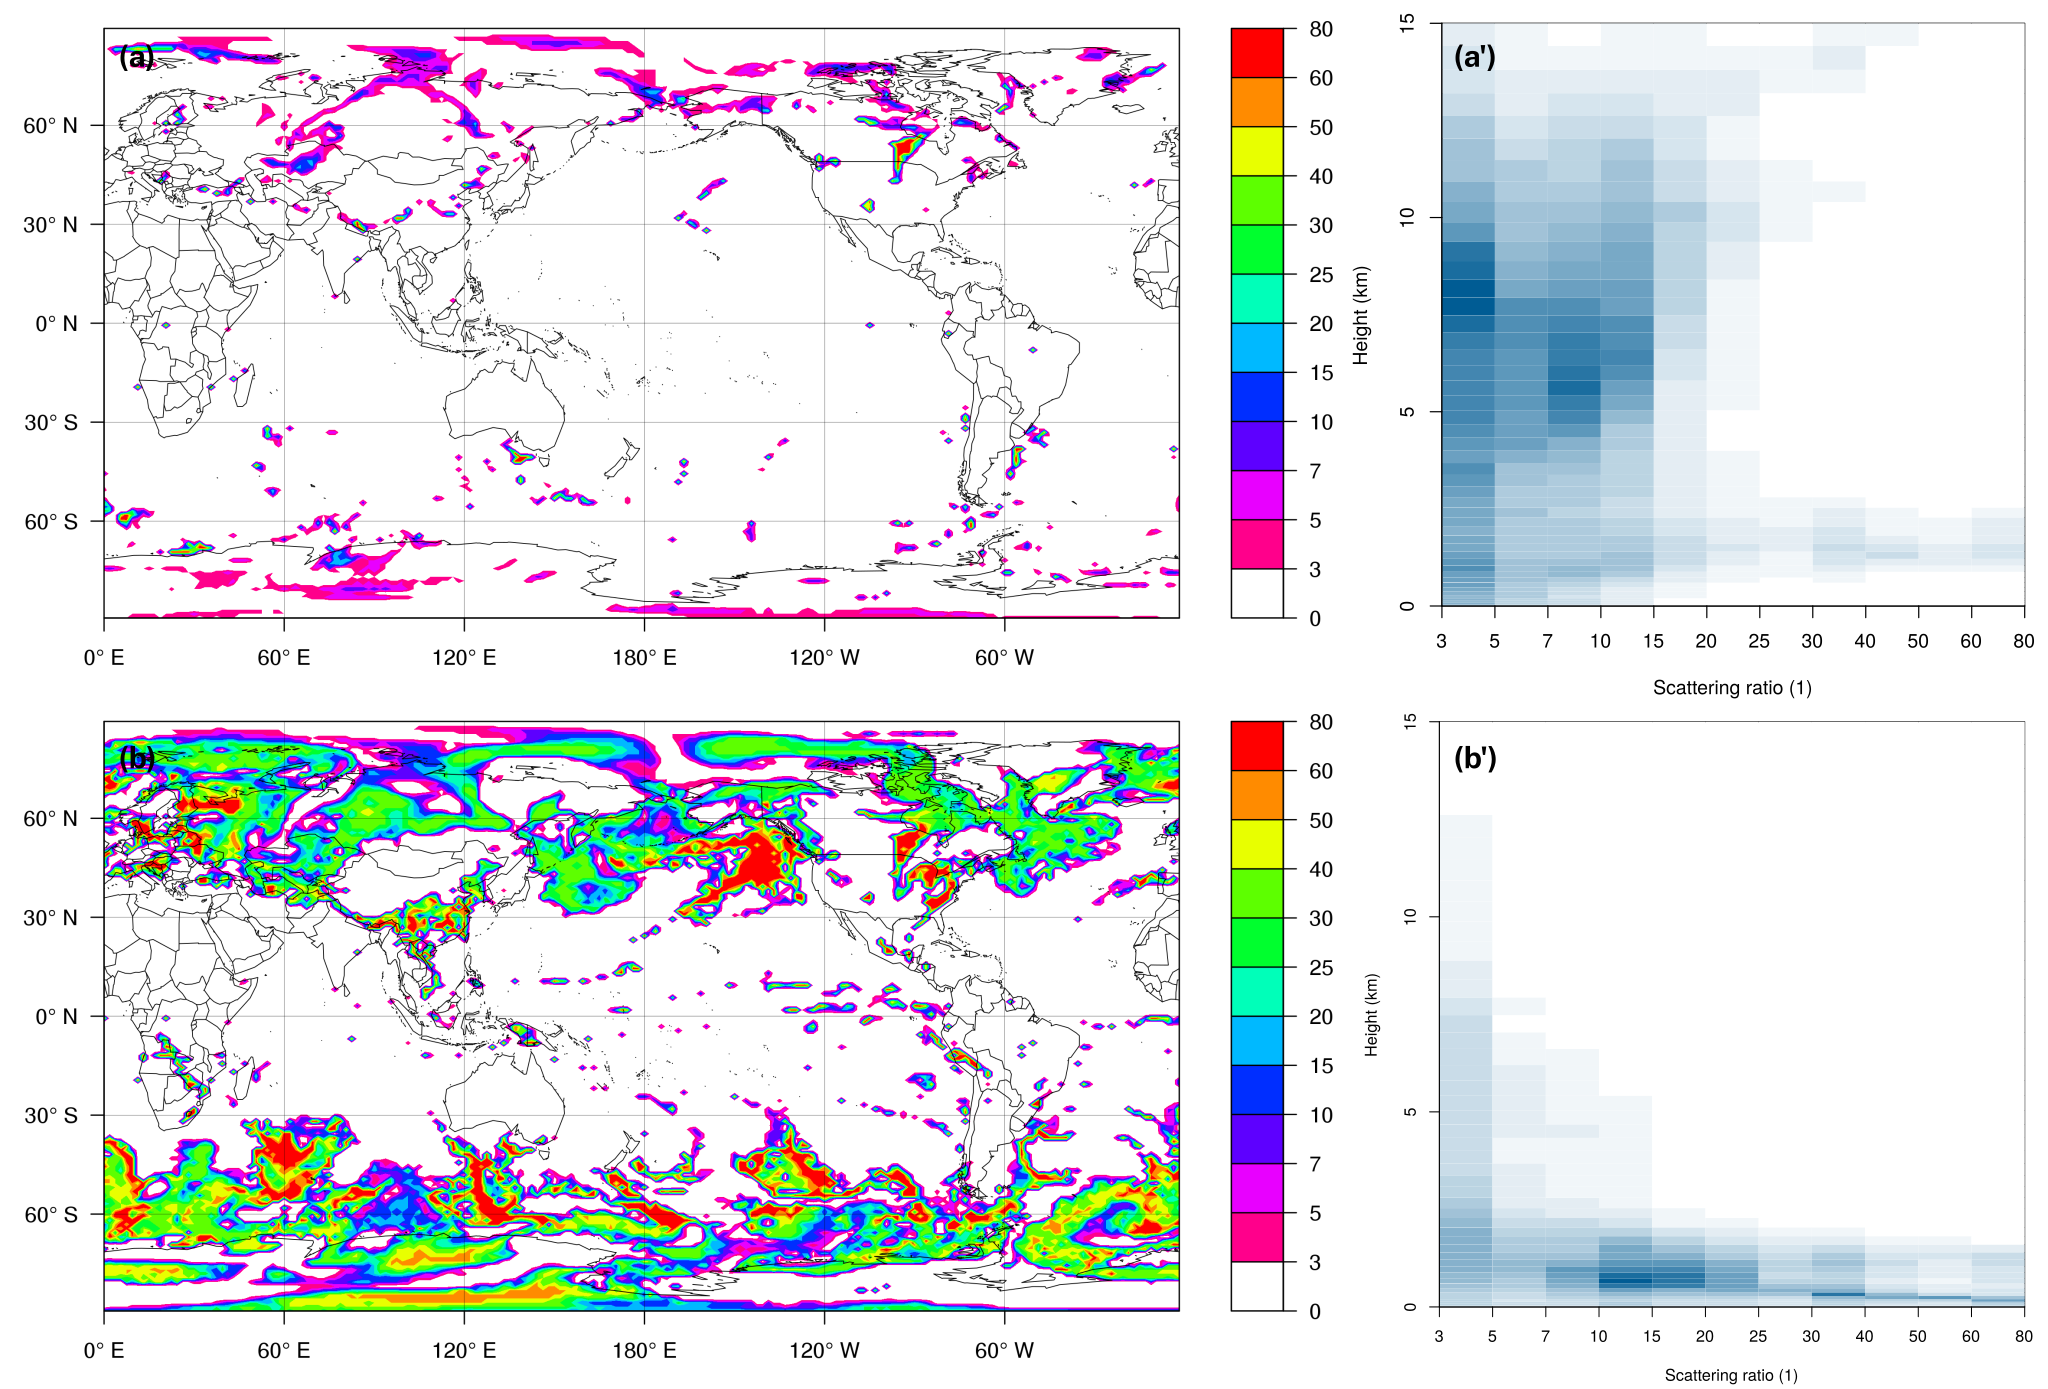
\includegraphics[width=\textwidth]{fig/space_vs_surface_lidar.png}
\caption[Spaceborne vs. surface lidar scattering ratio]{
\textbf{(a), (a')} Spaceborne vs. \textbf{(b), (b')} surface lidar scattering ratio
(SR) simulated based on the New Zealand Earth System Model (NZESM) output in
year 2017 at a lidar wavelength of 532 nm.
\textbf{(a), (b)} show SR at a model level corresponding to approximately 300 m
above sea level (ASL) over the sea, and \textbf{(a'), (b')} show an SR histogram by height.
}
\label{fig:surface-vs-spaceborne-lidar}
\end{figure}

Active satellite instruments are affected by signal attenuation by
optically thick
clouds (lidar), ground clutter (radar), and compared to passive instruments they have smaller spatial coverage,
shorter historical record and a small number of spectral bands, limiting their
ability to determine cloud microphysical properties \citep{noh2017,mace2018a,mace2018b,gettelman2020}.
In addition to spaceborne observations, ground-based and in situ
observations can provide an important complementary view of clouds from below.
Figure \ref{fig:surface-vs-spaceborne-lidar} shows that scattering ratio (SR)
(the ratio of total backscatter to molecular backscatter)
in the boundary layer measured by a lidar is much higher when measured by 
a ground-based lidar than a spaceborne lidar due to obscuration by higher-level
cloud.
Ground-based and in situ instruments include radars, ceilometers, lidars,
pyranometers, sky cameras, radiosondes, dropsondes, in situ aerosol measurements
(cloud condensation nuclei and ice nuclei) and airborne observations from
drones, weather balloons, kites and aircraft. These observations are logistically
difficult and expensive, and are generally sparse in the SO, with
limited time periods and limited historical records. The use of ground-based and
in situ observations alone for assessment of GCMs is difficult due to their
small representativeness of climatic conditions, and therefore there
is a risk of tuning the model to the specific conditions occurring during a
case study \citep{jakob2003}. Deployments on ships of opportunity can make these types
of observations more cost-efficient and common.

Different processing of observations from the same instrument can lead
to different results, for example the
GCM-Oriented CALIPSO Cloud Product (GOCCP) relative to the standard
Cloudsat--CALIPSO products \citep{chepfer2010}.
Different thresholds can be applied which define what 'cloud' is,
and cloud detection is affected by targeting a particular false alarm ratio,
such as 5\% as in the CloudSat--CALIPSO dataset \citep{hagihara2010}.
Probability of detection (sensitivity) then depends on the receiver operating
characteristic (ROC) curve, which in turn depends on instrument
noise. Instrument noise and bias can vary over lifetime of the instrument,
or between instruments of multi-instrument datasets such as ISCCP.
A problem with different processing
algorithms was noted by \cite{martucci2010}, who compared
manufacturer-supplied cloud base height (CBH)
determination between co-located Vaisala CL31 and Jenoptik CHM 15k ceilometers
and found a poor agreement, and developed a new algorithm for determining
CBH which leads to consistent height between the two instruments.

Due to the reasons outlined above, a combination of multiple satellite passive, active,
ground-based and in situ observations are needed to comprehensively assess
cloud climatology and biases. This has been also noted by other authors:
\cite{williams2017} evaluated cloud representation in the UK Met Office
Unified Model (UM) using a multi-dataset and multi-diagnostic approach, and
highlighted the
importance of using multiple instruments due to compensating errors in GCMs.
While use of single or combined satellite observations to assess model
performance is common in many studies,
combination of ground-based and spaceborne instruments is less common.
For example, \cite{muhlbauer2015} studied cirrus clouds using A-Train
observations (CloudSat, CALIPSO, MODIS, CERES), ground-based
Atmospheric Radiation Measurement (ARM) radar and aircraft observations.
\cite{zhang2017} performed a comparison of satellite and ground-based cloud
observations at an ARM site.

Comparison between models and observations cannot always be performed directly,
especially if observations do not produce fields equivalent to model quantities.
In such cases observations can be mapped to model fields by inversion algorithms,
but this may be unreliable
due to a large number of factors involved and a limited view of the instrument
(parts of the atmosphere obscured by clouds).
Conversely, model fields can be mapped to observations by instrument simulators,
and this approach has been used extensively in a number of studies.
Satellite simulators such as the Cloud Feedback Model Intercomparison Project (CFMIP) Observation Simulator Package (COSP)
\citep{bodas-salcedo2011} solve the problem
by transforming model fields to observed fields, which can then
be compared directly or statistically.

We provide a further literature review in Chapter 2.

\section{Objectives}
\label{sec:objectives}

Our objectives are aligned with the New Zealand Deep South National
Science Challenge (DSC), whose mission is to \textit{`enable New Zealanders to adapt,
manage risk, and thrive in a changing climate'}, and is
broadly in line with the current international research in the area
such as the Southern Ocean Clouds
Radiation Aerosol Transport Experimental Study (SOCRATES) \citep{mcfarquhar2014}.
Here, we focus on complementing other studies evaluating
representation of clouds, aerosols and cloud-aerosol interaction in the SO,
but also taking into consideration the Southern Hemisphere and global processes,
with a particular focus on utilising in situ measurements
available from intensive observation periods (IOPs), complemented by land-based
stations. For this
purpose the COSP simulator needs to be extended to support these
instruments. A ground-based observations need to be
complemented by satellite observations, especially the global radiation budget
measurements by CERES.
Other diagnostic means include
case studies, by which we can ensure that any improvements are due to
the right physical reasons rather than just improving statistics by mutually
compensating model errors. Our particular focus is therefore on linking
observed biases to model processes. 
We shall try to evaluate specific deficiencies in the NZESM subgrid-scale
parametrisations affecting clouds and radiative transfer, in order to
determine the relative importance of cloud macrophysical and microphysical
characteristics in the observed biases. This has been explored to some extent
by other authors, but not always in the context of the UM or the NZESM,
where the causes can be different.
While our focus is on evaluation of the NZESM, contrasting with other
models, such as atmospheric reanalyses is useful.
We shall focus on biases in the SO and the
Antarctic, but pay attention to any processes relevant to the Southern
Hemisphere and globally.
Adjacent to our study will be development of a publicly-available dataset
of in situ observations in the SO based on previous and new SO voyages
and permanent stations collected by the University of Canterbury and our
collaborators.
Our main objectives are outlined below:

\begin{enumerate}
\item Participate on SO IOPs
with the aim of collecting atmospheric observations for model evaluation.
\item Collate and post-process the existing and new SO in situ datasets.
\item Extend the COSP lidar simulator with a ceilometer and ground-based lidar
simulator for instruments deployed on the SO voyages.
\item Use in situ and satellite observations in conjunction with the lidar simulator
to evaluate SO cloud biases in the NZESM.
\item Perform experimental simulations of the NZESM with the aim of
improving the simulation of SO clouds relative to the observations.
\end{enumerate}

\section{Methods}

Achieving our objectives will require a number of modelling and
observational resources. As outlined here and discussed in
a greater detail in Chapter 2, 3 and 4, these include access to the model output
and
code of the NZESM, the COSP simulator, publicly-available reanalyses,
 in situ SO observations and publicly-available
satellite datasets.

\subsection{New Zealand Earth System Model}

The NZESM is an actively developed branch of HadGEM/UKESM, with the
aim of improving the atmosphere, ocean and cryosphere simulation affecting
Aotearoa/New Zealand
\citep{williams2016}. Development is done by the National Institute of Water and
Atmospheric Research (NIWA) in Wellington and the University of Canterbury.
The NZESM is a fully coupled atmosphere-ocean model, including land surface
and sea ice. The parent model UKESM \citep{walters2017} is planned to participate
in the 6th Climate Model Intercomparison Project (CMIP6) \citep{eyring2016,meehl2014},
which shall eventually contribute to the upcoming
Intergovernmental Panel on Climate Change (IPCC) 6th
Assessment Report (AR6). Participation of the NZESM in the CMIP6 is currently not
envisioned, although any improvements achieved will be continuously contributed
to the parent model.

Apart from a standard free-running mode, it is possible to run the NZESM
in a nudged mode, continuously modulated by observed meteorological
conditions using the ERA-Interim reanalysis \citep{dee2011} and prescribed SST and sea ice
by the HadISST dataset \citep{rayner2003}.
A nudged run can be useful for comparison with instantaneous values of
observational data taken during the simulated period,
as opposed to long-term statistics. The model fields can be exported
at arbitrary intervals down to the model time step of 20 minutes.

\subsection{CFMIP Observation Simulator Package}

COSP \citep{bodas-salcedo2011} is a satellite instrument simulator package
for atmospheric model evaluation developed as part of
the CFMIP \citep{bony2011},
whose purpose is to generate pseudo-measurements and statistics from model fields, which can
then be compared to real
measurements. A direct comparison without a simulator is often not possible
due to a limited field of view (FOV) of the instrument and attenuation by atmospheric
constituents (clouds, aerosols, gases), which is a wavelength-dependent process.
COSP was utilised in evaluation of GCMs in the
Coupled Model Intercomparison Project Phase 5 (CMIP5) \citep{taylor2011}.
COSP contains multiple simulators of different instruments:
ISCCP, MODIS, MISR, CloudSat, CALIPSO, a MilliMeter-wavelength Cloud Radar
(MMCR)/Ka-Band ARM Zenith Radar (KAZR) ground-based radar
and the Radiative Transfer for Television Infrared Observation Satellite (TIROS)
Operational Vertical Sounder (TOSV) (RTTOV).
Notably, radar observations are simulated by the QuickBeam simulator
\citep{haynes2007} and lidar (CALIPSO) observations are simulated
by the Active Remote Sensing Simulator (ACTSIM) \citep{chepfer2008}. In general, these may need
to be tuned for any particular instrument being simulated due to different
wavelengths, signal modulation, view and error characteristics.
COSP allows for comparison of instrument quantities
(backscatter, radar reflectivity), or derived products
(cloud top/base, cloud phase, ...) between the model and observations.
An exact co-located comparison is limited by the relatively low spatial and
temporal resolution
of GCMs, and pseudo-observations need to be made on subcolumns generated by
a cloud generator. Algorithms for calculating derived products are generally not
available, and datasets such as CALIPSO-GOCCP were developed for the purpose
of comparison of equivalent quantities from observations and the simulator
\citep{chepfer2010}.
COSP can be run either online (inside the model) or offline,
when fields from a model are provided to COSP after completing the simulation.
Running the simulator offline allows for rapid modification
and testing of code. Cloud overlap in COSP is treated by the Subgrid Cloud Overlap Profile Sampler
(SCOPS) \citep{webb2001}, which generates subcolumns based on the grid cell
cloud fraction and precipitation fluxes. Either random or maximum-random cloud overlap
\citep{geleyn1979,ritter1992} is assumed,
whereby cloud in the adjacent layers overlaps maximally, and cloud separated
by clear layers overlaps randomly.

ACTSIM is a lidar simulator integrated in COSP
\citep{chepfer2008,chiriaco2006}. In the current implementation it simulates a
spaceborne lidar with a wavelength of 532 nm, aimed at simulating the CALIOP
instrument on CALIPSO. The simulator produces attenuated volume backscatter
coefficient, which can be compared directly with measurements from a lidar.
Support for a ground-based ceilometer such as Lufft CHM 15k or Vaisala CL51
will require modification of ACTSIM. Firstly, the viewpoint from
the ground means that the lidar signal passes through atmospheric layers in a reversed
order relative to what is assumed for a spaceborne lidar. Secondly,
wavelength of our instruments is different from CALIOP (1064 nm and 910 nm),
which requires re-calculation of the Mie and Rayleigh scattering coefficients.

\subsection{In situ observations in the Southern Ocean}

\begin{figure}[t]
\centering
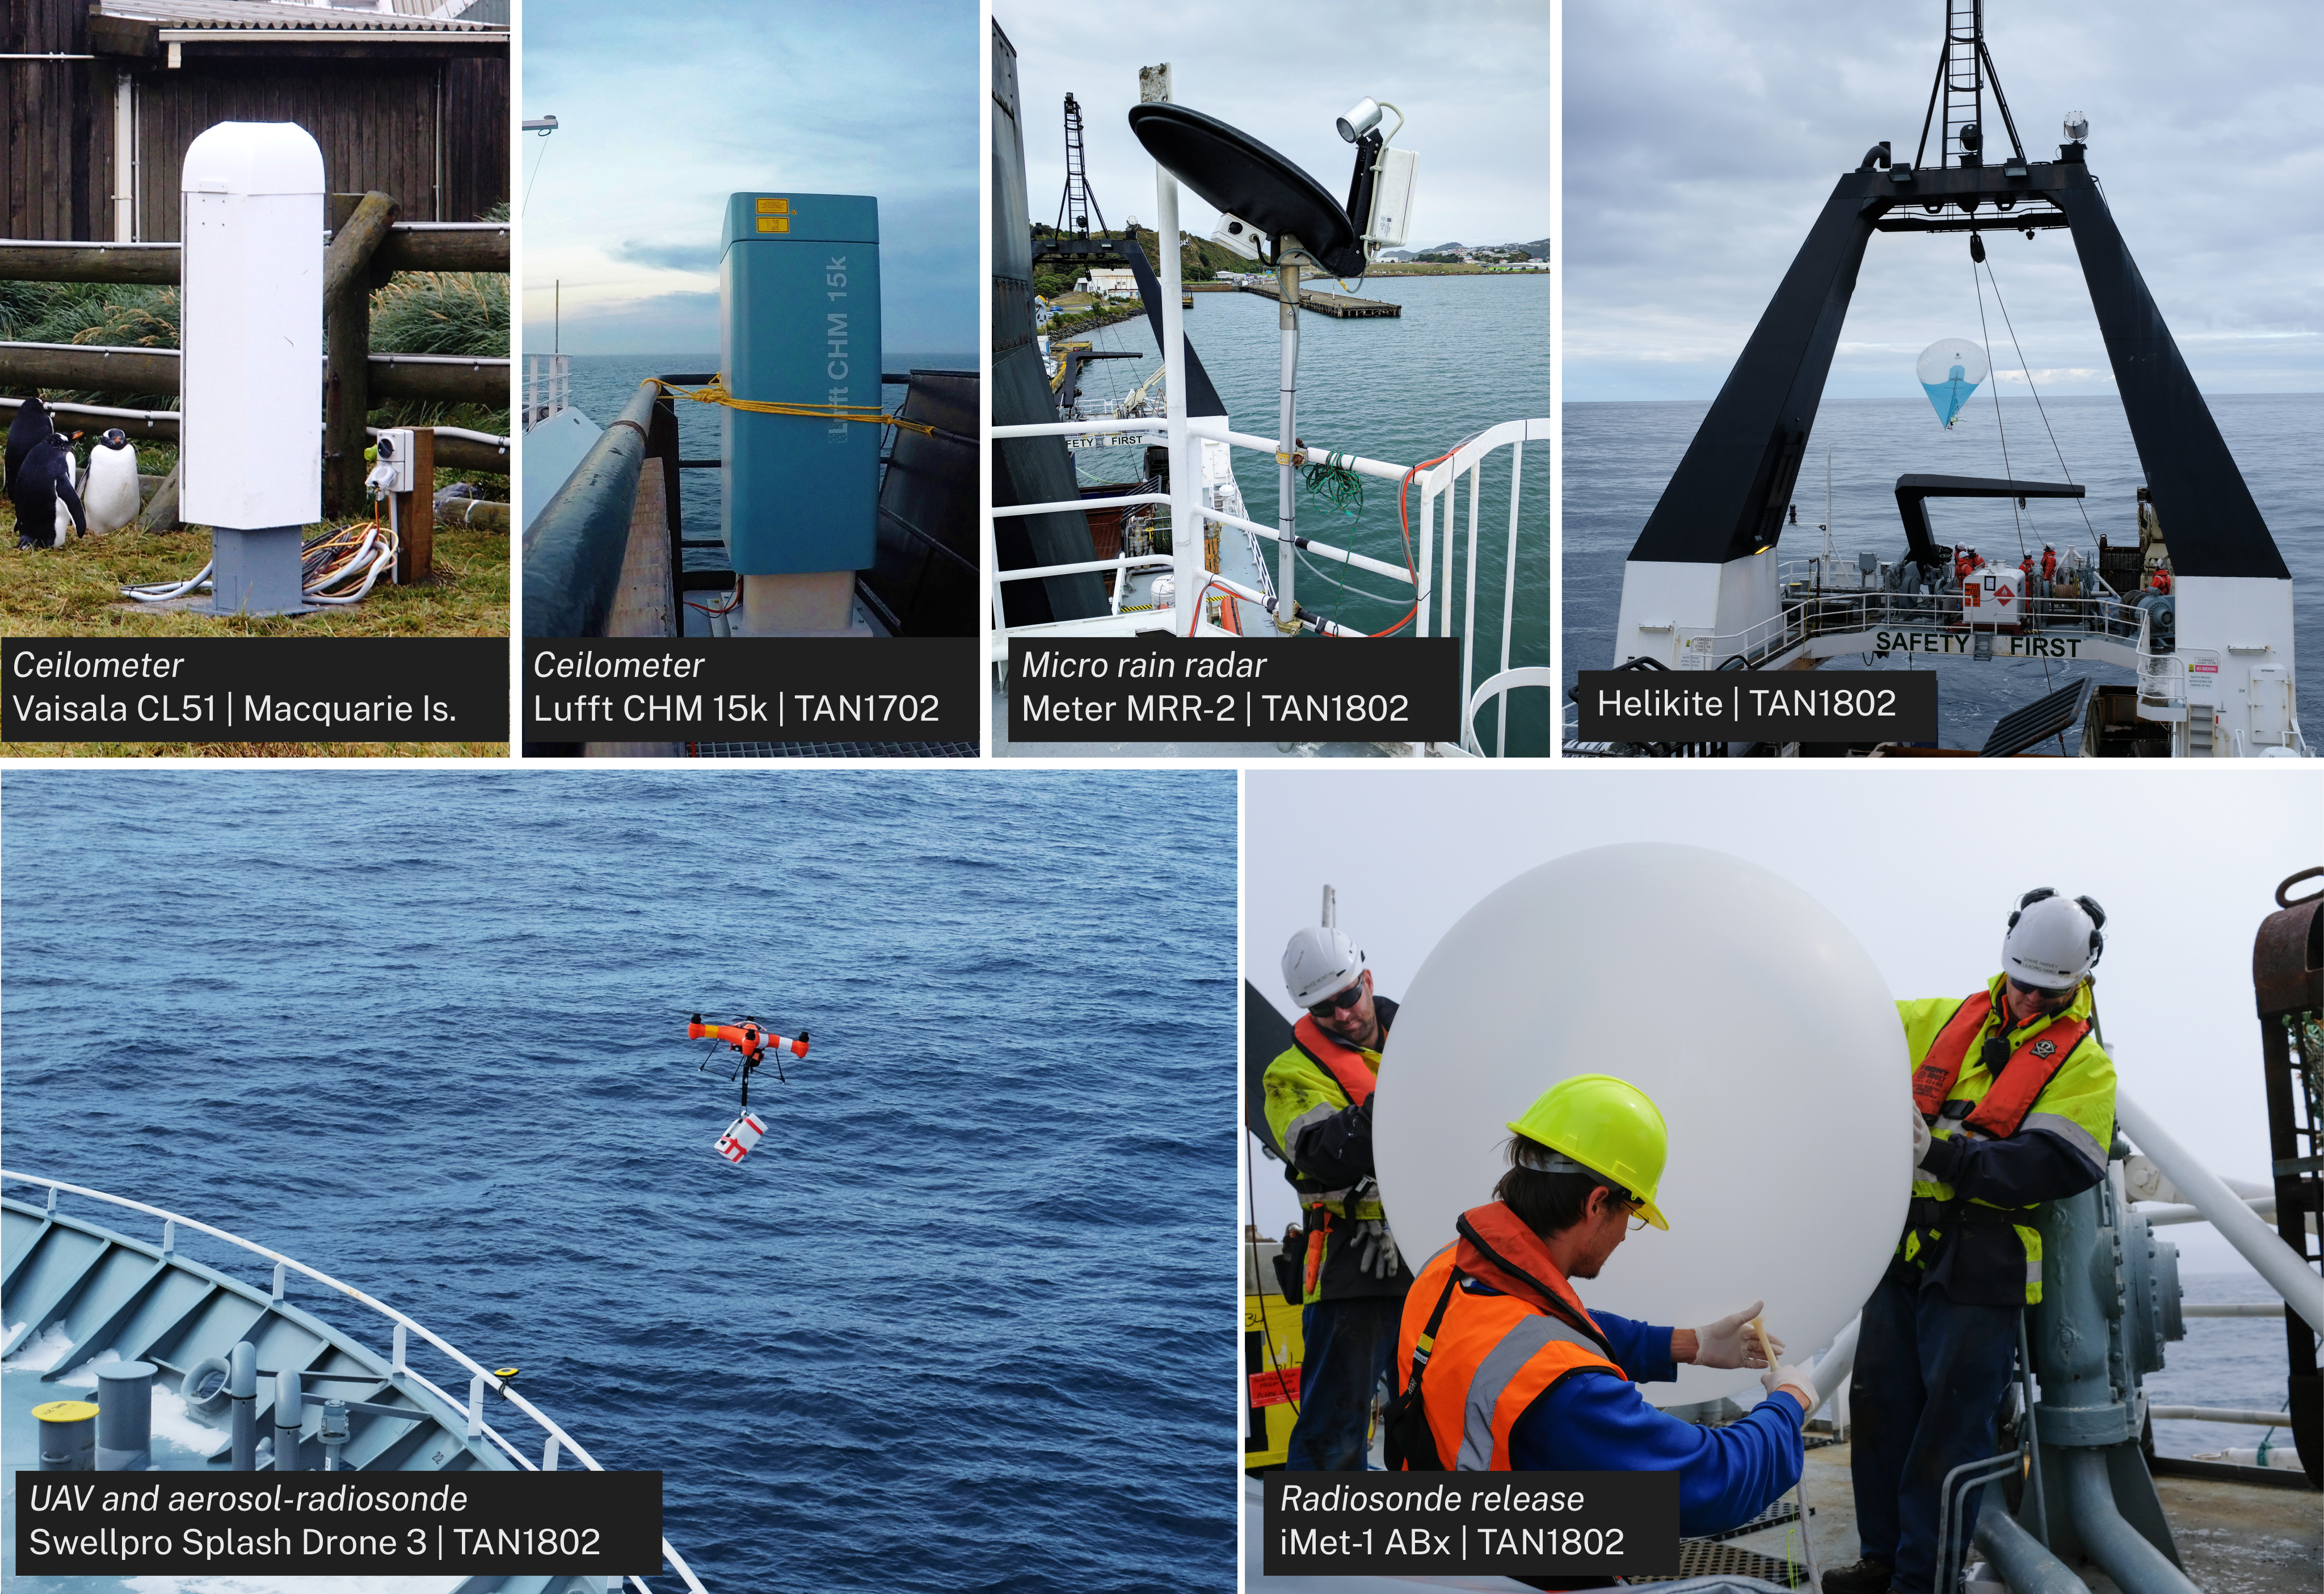
\includegraphics[width=\textwidth]{fig/instruments.jpg}
\caption{
Instruments deployed on Southern Ocean voyages and stations.
}
\label{fig:instruments}
\end{figure}

In situ SO observations are essential for improving the model SO biases.
A set of SO datasets have been collected by the University of Canterbury
and partner organisations by deploying our instruments on a number
of voyages of opportunity as well as conducting IOPs:

\begin{itemize}
\item \textit{Aurora Australis} voyages to Casey, Davis and Mawson, Antarctica (2015--2016).
\item Macquarie Island station (2016--2018).
\item HMNZS \textit{Wellington} voyages to the Ross Sea (2016).
\item RV \textit{Nathaniel B. Palmer} voyage NBP1704 to the Ross Sea (2017).
\item RV \textit{Tangaroa} voyages TAN1502, TAN1503 (2015), TAN1702 (2017) and TAN1802 (2018)
to the Ross Sea, Chatham Islands, the Campbell Plateau and the Ross Sea, respectively.
\end{itemize}

\noindent
The author participated on field measurements on the TAN7102 and TAN1802 voyages and the deployments
on the HMNZS \textit{Wellington} and the NBP1704.
In addition to the datasets outlined above we have access to a set of
ceilometer and lidar observations from the following land-based locations in
Aotearoa/New Zealand:

\begin{figure}[t]
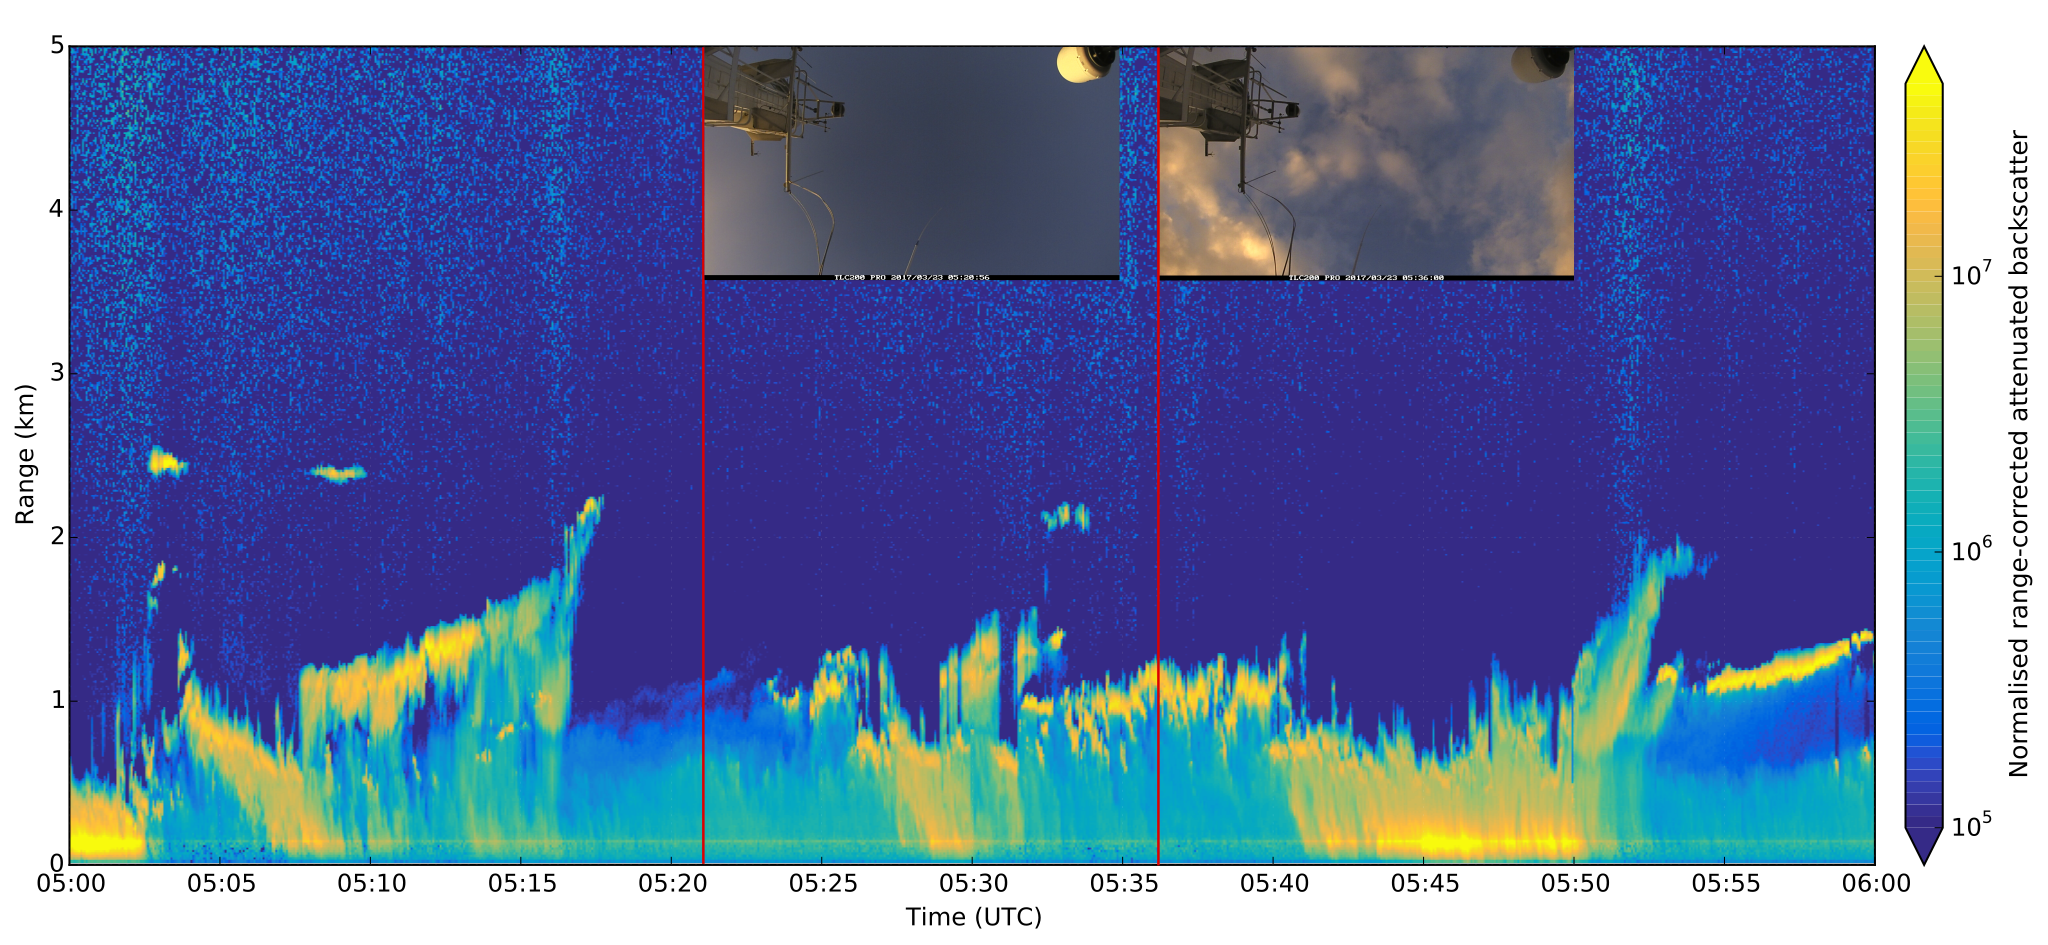
\includegraphics[width=\textwidth]{fig/chm15k_profile.png}
\caption[Lufft CHM 15k ceilometer volume backscattering coefficient profile plot]{
A Lufft CHM 15k ceilometer volume backscattering coefficient profile plot
and corresponding sky camera images collected on the TAN1702 voyage
on 23 March 2017.
}
\label{fig:chm15k-profile}
\end{figure}

\begin{itemize}
\item \textbf{Cass}, a deployment of a Vaisala CL51 ceilometer at a station in the
Southern Alps, Aotearoa/New Zealand.
\item \textbf{Lauder}, a dataset of a Sigma Space MiniMPL lidar and a Vaisala CL31
ceilometer observations at a station in Aotearoa/New Zealand made available by NIWA.
\item \textbf{Christchurch}, a deployment of a Lufft CHM 15k and a Sigma Space MiniMPL on the
Ernest Rutherford building of the University of Canterbury, Aotearoa/New
Zealand.
\end{itemize}

Observations collected on the voyages include remote sensing with ceilometers and lidars,
a micro rain radar, radiosonde profiles, automatic weather station (AWS) data (temperature, relative humidity,
wind, SST, radiometer...), UAV and tethered balloon soundings and
aerosol concentration (Fig. \ref{fig:instruments}.
Below, we briefly describe the instruments.

\textit{Lufft CHM 15k} is an IR ceilometer operating at a single wavelength of
1064 nm, which makes it suitable for observation of cloud droplets and
ice particles of similar size and boundary layer aerosol.
The primary purpose of a ceilometer
is observation of CBH, although other atmospheric features
such as boundary layer height, visibility, precipitation and multiple
cloud layers can be detected as well using a suitable algorithm. The
primary measured quantity is attenuated volume backscattering coefficient
$\beta$ (km$^{-1}$sr$^{-1}$), which
can also be used for a direct comparison with a ceilometer simulator.
The instrument allows for an easy deployment
in adverse conditions, such as on ships.
The ceilometer records data in the NetCDF format \citep{rew2006},
which makes it easy
for processing by various data analysis tools.
The averaging period of the instrument is 2 s. This provides spatiotemporal
resolution much greater than a GCM. Averaging over longer time periods can be applied to improve the signal-to-noise ratio (SNR).

\textit{Vaisala CL51} is an IR ceilometer operating a
wavelength of 910 nm. Similar to Lufft CHM 15k, it is suitable for observation
of cloud droplets and ice particles. The averaging period is 6 s.
The firmware contains onboard detection of multiple cloud layers and
visibility by a standard algorithm and a Sky Condition Algorithm (SCA).
Two-dimensional backscatter profiles are recorded in ASCII-encoded data files.

\textit{Metek MRR-2} is a micro rain radar, operating at a microwave frequency of
24.230 GHz, i.e. wavelength of 12.38 mm. The wavelength makes it suitable
for observation of liquid and ice precipitation. This instrument can
be used alongside the Vaisala CL51 instrument to detect period of time with
precipitation and rain rate. A Metek MRR-2 was deployed on the TAN1702, TAN1802
and HMNZS \textit{Wellington} voyages.

A sky camera was used as an ancillary instrument providing a visual
perspective of the atmospheric conditions (type of cloud, fog,
precipitation), as well as a primary instrument for determining cloud fraction.
Our deployments included
an off-the-shelf time lapse camera Brinno BCC200 (as a low-cost but
satisfactory solution) and a fisheye-lens camera.
The sampling period can be chosen from a wide range of values; we have
determined that a 5-minute interval is sufficient.
Figure \ref{fig:chm15k-profile} shows an example backscatter profile plot
from the TAN1702 voyage, combined with sky camera images. 
In addition to CBH, these measurements provide a wealth
of information about the cloud type, the vertical extent, optical thickness,
precipitation, fog and boundary layer aerosol. Some of these, as well
as satellite cloud observations in the Ross Sea region, were analysed
by co-authored studies: \cite{klekociuk2018,jolly2018,hartery2020a,hartery2020b}.

Preliminary analysis of multiple voyage datasets indicates that low cloud
below 2 km constitutes the majority of cloud in the summertime in the SO
(Fig. \ref{fig:cbh}). Preliminary results from the TAN1802 voyage also
show a very high cloud fraction of 94\% and a strong peak of boundary layer
cloud below 1 km above sea level (ASL) (Fig. \ref{fig:tan1802-stats}a), the predominance
of stratus (52\%) and stratocumulus (30\%) clouds (Fig. \ref{fig:tan1802-stats}b), predominantly
near-zero SST (Fig. \ref{fig:tan1802-stats}c) and near-surface air temperature below SST
(Fig. \ref{fig:tan1802-stats}d, e). These results suggest a cold boundary layer
destabilised by relatively warm SST and subsequent formation of
low stratus and stratocumulus cloud.

\begin{figure}[t]
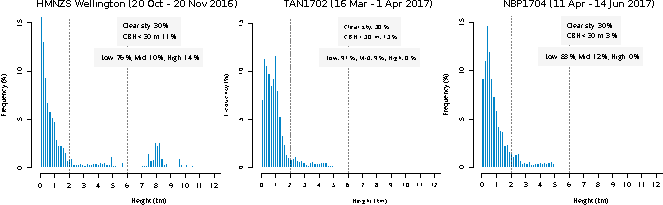
\includegraphics[width=\textwidth]{fig/cbh.pdf}
\caption[Cloud base height distribution]{
Cloud base height distribution on the HMNZS \textit{Wellington} 2016, TAN702 and NBP1704
voyages derived with a Lufft CHM 15k ceilometer observations (as determined by
the instrument's firmware).
}
\label{fig:cbh}
\end{figure}

\begin{figure}[t]
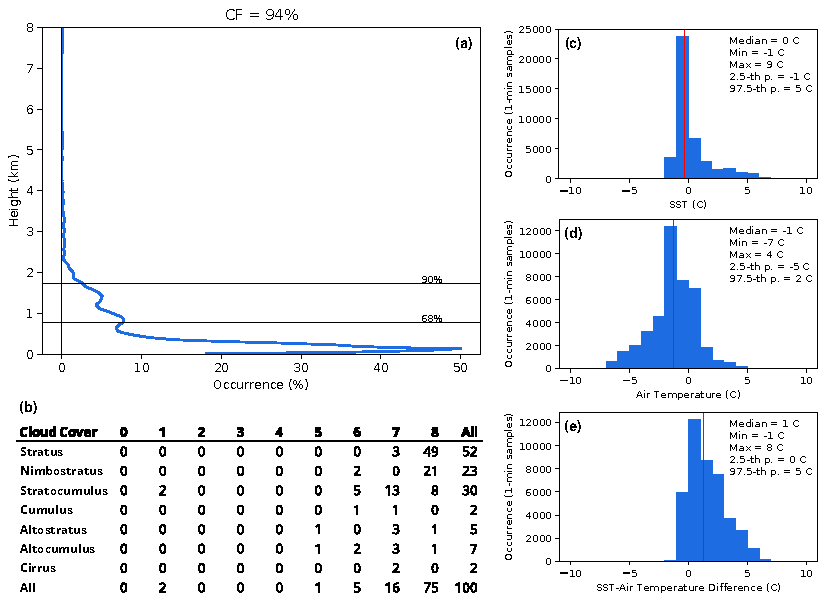
\includegraphics[width=\textwidth]{fig/tan1802_stats.pdf}
\caption[Statistics calculated from observations collected on the TAN1802 voyage]{
Statistics calculated from observations collected on the TAN1802 voyage.
\textbf{(a)} cloud occurrence as a function of height, the 68-th and
90-th percentiles and the total cloud fraction (CF) calculated from a Lufft CHM 15k ceilometer observations.
\textbf{(b)} cloud type and cloud cover (octas) occurrence
in \% calculated from human observations. Histograms of \textbf{(c)} sea surface temperature (SST), \textbf{(d)} air temperature
and \textbf{(e)} SST - air temperature calculated from the automatic
weather station (AWS) data.
}
\label{fig:tan1802-stats}
\end{figure}

\subsection{Satellite radiation budget observations}

Earth radiation budget (ERB) observations are central for assessment and development
of GCMs. LEO satellite observations of TOA SW and longwave (LW) fluxes
have been performed starting with the Nimbus satellite series in 1970s
\citep{smith1977}, followed by the Earth Radiation Budget Satellite (ERBS) and NOAA
satellites in 1980s \citep{barkstrom1984}, the Scanner for Radiation Budget (ScaRaB)
project on on Meteor-3 and Resurs-01/4 LEO satellites in 1990s \citep{kandel1994}
and the
CERES instruments on a number of LEO satellites from late 1990s
to the present day \citep{wielicki1996}. Geosynchronous satellite measurements
have the advantage of continuous temporal sampling, but cannot provide a
good angular resolution and observations at high polar latitudes. They have,
however, been utilised as part of the Geostationary Earth Radiation Budget (GERB)
project.
The National Institute of Standards and Technology Advanced Radiometer (NISTAR)
instrument on the Deep Space Climate Observatory (DSCOVR) satellite in L1 Lagrangian point provides continuous
measurements of the sunlit part of the Earth \citep{khlopenkov2017}. It has,
however, not been used
as extensively as earlier satellite observations. Global radiation balance
is one of the most commonly adjusted properties of GCMs
\citep{hourdin2017,schmidt2017}. It is vital for GCMs to simulate accurate
spatiotemporal variability of the radiation budget, as deviations can cause
shifts in circulation patterns such as the polar fronts and
the inter-tropical convergence zone (ITCZ).

CERES are instruments measuring the ERB,
deployed on multiple satellites:
TRMM (1997--2015), Terra (2000--present), Aqua (2002--present), Suomi NPP (2011--present) and JPSS-1
(2017--present) \citep{damadeo2017}. They are
considered to provide the most reliable measurements of radiation budget,
although they are limited by the necessity of temporal (diurnal) and angular
interpolation \citep{smith2011}.
Recent version of the CERES Energy Balanced and
Filled (EBAF) dataset (Edition 4.0) has been found to decrease
clear-sky TOA SW flux in the SO region in January by up to 15 Wm$^{-2}$
in summer compared to the previous version \citep{loeb2017},
which may affect previous results and should be taken into consideration in
future analysis.

The Geostationary Earth Radiation Budget (GERB) project involves ERB instruments
on Meteosat Second Generation (MSG) GEO satellites \citep{harries2005}.
Measurements began in 2002 on MSG-1 and continue to the present day.
Both SW and LW bands are available. The advantage of GERB
over CERES is its continuous temporal and spatial coverage in its FOV
\citep{sandford2003}. However, it does not provide full spatial coverage
(polar latitudes and longitudes outside of its FOV).
GERB has been used for correction of CERES temporal interpolation
(CERES geostationary method), resulting in difference in excess of 25 Wm$^{-2}$
over marine stratus and land convection relative to uncorrected data
(CERES-only) \citep{doelling2013}. It is therefore important to consider
the effect of temporal interpolation when comparing regional ERB with a GCM.
Because high latitudes are not observed by GEO satellites, this correction
cannot be done for latitudes over 60$^{\circ}$. This is compensated by the high-revisit
frequency of the CERES-carrying satellites at the poles.

%\begin{figure}
%\begin{subfigure}[b]{0.5\textwidth}
%\textbf{a}\\
%\includegraphics[width=\textwidth]{img/sr_hist_2007_spaceborne.pdf}
%\end{subfigure}
%\begin{subfigure}[b]{0.5\textwidth}
%\textbf{b}\\
%\includegraphics[width=\textwidth]{img/sr_hist_2007_surface.pdf}
%\end{subfigure}
%\caption{
%\textbf{Simulated scattering ratio histogram
%(global, year 2007 of NZESM simulation).}
%\textbf{a,} Surface lidar (532 nm),
%\textbf{b,} Spaceborne lidar (532 nm).
%}
%\label{fig:hist}
%\end{figure}

\subsection{Auxiliary software}

As part of the observational data processing work we developed
open source tools for transforming the native instrument data formats to
the more commonly used NetCDF and HDF formats:

\begin{itemize}
\item \textbf{cl2nc}\footnote{\url{https://github.com/peterkuma/cl2nc}.}, a tool for converting Vaisala CL51
ceilometer data to NetCDF4.
\item \textbf{mrr2c}\footnote{\url{https://github.com/peterkuma/mrr2c}.}, a tool for converting
Metek MRR-2 radar data to HDF5.
\item \textbf{mpl2nc}\footnote{\url{https://github.com/peterkuma/mpl2nc}.}, a
tool for converting Sigma Space MiniMPL lidar data to NetCDF4 and applying
dead time, overlap and afterpulse calibration.
\end{itemize}

\noindent
These tools were made publicly available on the code collaboration network
GitHub.

\section{Outline of the thesis and author's contributions}

This thesis consists of the Introduction (Chapter 1), three research chapters
(Chapter 2, 3 and 4) and Conclusions and further work (Chapter 5). The three
research chapters are accepted for publication (Chapter 2),
in review (Chapter 3) and a manuscript in preparation (Chapter 4).
The author of this thesis is the primary author of the three manuscripts.
Chapter 2 provides a comprehensive literature review on the central topic
of this thesis: model cloud biases in the SO. In Chapter 2 we evaluate
SO cloud in a nudged run of the GA7.1 and MERRA-2 in comparison
with a collection of SO voyage observations. In Chapter 3 we
describe a new ground based lidar processing and simulator framework.
In Chapter 4 we describe and evaluate an experimental run of the UM11.4 aimed at
improving representation of boundary layer cloud in the SO.
As of May 2020, Chapter 2 was accepted for publication in the Atmospheric
Chemistry and Physics (ACP) \citep{kuma2020a}. Chapter 3 was submitted to the
Geoscientific Model Development (GMD) and is due to be in review
in Geoscientific Model Development Discussions (GMDD) after a minor revision \citep{kuma2020b}.
Co-authored published studies related to this thesis are: \cite{jolly2018}
(published in ACP), \cite{klekociuk2018} (published in Deep Sea Research Part II: Topical Studies in Oceanography), \cite{hartery2020a}
(published in Journal of Geophysical Research: Atmospheres) and
\cite{hartery2020b} (submitted to Geophysical Research Letters).
